\part{Celda Universal}
\section{Introducción}
En esta sección se busca realizar un filtro \textit{Notch} que cumpla una determinada plantilla y que sea implementada con una celda universal. 

\section{Plantilla}

En la Tabla \ref{tab:ej4_plantilla} se puede observar la plantilla del filtro \textit{Notch}. Como parámetros a destacar esta la frecuencia del \textit{notch} ($f_0$) a $30kHz$ con una profundidad mayor a $50 dB$.

\begin{table}[h!]
    \centering
    \begin{tabular}{|c|c|}
    \hline
    $f_0$                      & 30kHz                             \\ \hline
    Notch Depth                        & $> 50 dB$                           \\ \hline
    $\Delta f_a$                       & 600Hz                             \\ \hline
    $\Delta f_p$                        & 13Hz                              \\ \hline
    $A_a$                              & 40dB                              \\ \hline
    $A_p$                              & 6dB                               \\ \hline
    $G$                              & [-3:3]dB                               \\ \hline
    $|Z_{in}(f)|$                    & $>50k\Omega$                               \\ \hline
  
    \end{tabular}
    \caption{Plantilla}
    \label{tab:ej4_plantilla}
    \end{table}


\section{Cálculos teóricos}
En esta sección se utiliza la aproximación de Chebychev II para diseñar el filtro. En primer lugar, se deben calcular $f^-_a$, $f^+_a$, $f^-_p$ y $f^+_p$. Las mismas son calculadas utilizando las siguientes ecuaciones:
\begin{displaymath}  f^2_0 = f^-_a f^+_a = f^-_p f^+_p \end{displaymath} 
\begin{displaymath}  \Delta f_a = f^-_a - f^+_a \end{displaymath}     
\begin{displaymath}  \Delta f_ p= f^-_p - f^+_p \end{displaymath} 

Gracias a estas ecuaciones y a la plantilla, se obtiene:

\begin{displaymath}  f^-_a = 29701 Hz \end{displaymath}     
\begin{displaymath}  f^+_a= 30301 Hz \end{displaymath} 
\begin{displaymath}  f^-_p= 24196 Hz \end{displaymath} 
\begin{displaymath}  f^+_p= 37196 Hz \end{displaymath} 


Se cargan estos últimos resultados y la plantilla en un programa de aproximación. Los resultados muestran que para implementar el filtro se deben tener dos etapas donde ambas son filtros notch. En la Figura \ref{ej4_diagrama_polos_ceros} se pueden ver el diagrama de polos y ceros que deben tener las etapas del filtro. Nótese que, ambos pares de ceros se encuentran sobre el eje $j\omega$. Las frecuencias de los polos y ceros son las siguientes:

\begin{displaymath}  f_{p1} = 24479 Hz \end{displaymath}     
\begin{displaymath}  f_{p2}= 367643.91 Hz \end{displaymath} 
\begin{displaymath}  f_{z1}= 29848 Hz \end{displaymath} 
\begin{displaymath}  f_{z2}= 30151 Hz \end{displaymath} 


\begin{figure}[h!]                                                       
    \centering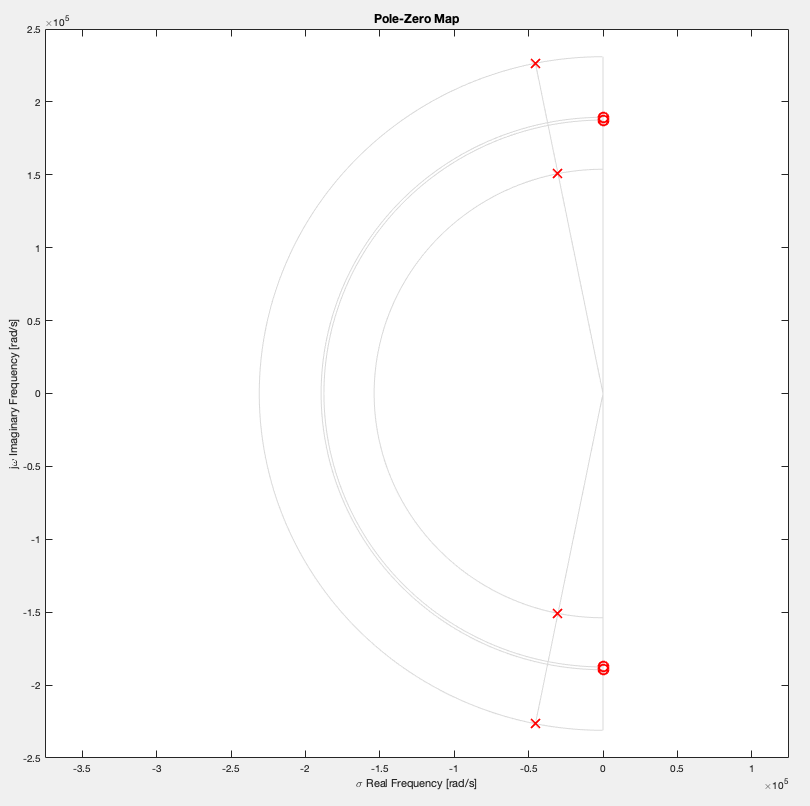
\includegraphics[width=0.6\textwidth]{../Ex4/Resources/ej4_diagrama_polos_ceros.png}
    \caption{Diagrama de polos y ceros}
    \label{ej4_diagrama_polos_ceros}
    \end{figure}

Donde los sufijos $p$ y $z$ representan polos y ceros respectivamente. Ademas, ambas etapas tienen $Q = 2.54$. Con toda esta información es posible armar las funciones transferencias de las dos etapas. La función transferencia de la primera etapa sera $H_1(s)$ y la segunda sera $H_2(s)$. Para poder armarlas se debe primero agrupar los pares de polos y ceros. Es decir, se debe decidir que polo se asigna con cual cero. Una regla simple que optimiza el rango dinámico del filtro es agrupar los polos con los ceros que estén mas próximos. Es fácil demostrar (observando la 
Figura \ref{ej4_diagrama_polos_ceros}) que $p1$ esta mas cerca de  $z1$ y $p2$ esta mas cerca de $z2$. Entonces, las funciones transferencias son:

\begin{equation} H_1(s) = k\frac{s^2 + w^2_{z1}}{s^2 + s\frac{w_{p1}}{Q} + w^2_{p1}} \label{ej4_h1}\end{equation}
\begin{equation} H_2(s) = k\frac{s^2 + w^2_{z2}}{s^2 + s\frac{w_{p2}}{Q} + w^2_{p2}} \label{ej4_h2}\end{equation}

Donde $k$ representa la ganancia asignada a cada etapa. Esta ganancia es util para asegurar que las señales se mantengan por debajo de los limites de saturación del amplificador operacional utilizado para hacer la etapa. Sin embargo, como se ve en la sección \textit{Diseño}, se define $k=1$. 

Por ultimo, se debe definir el orden de las etapas. Es decir, como las etapas se implementan en cascada, se debe definir en que orden se implementan $H_1(s)$ y $H_2(s)$. La regla de decisión es implementar las etapas de manera que las de menor $Q$ estén primero. Pero como en este caso ambas etapas tienen el mismo $Q$, se define arbitrariamente que la primera etapa sea $H_1(s)$.


Como (\ref{ej4_h1}) y (\ref{ej4_h2}) son de la misma forma, es de utilidad tener una función transferencia genérica  para usar en la sección de \textit{Diseño}. La misma se muestra a continuación:

\begin{equation} H(s) = k \frac{s^2 + w_z^2}{s^2 + s\frac{w_p}{Q} + w^2_p} \label{ej4_transferencia_notch}\end{equation}


Para finalizar la sección se muestran las atenuaciones de ambas etapas por separado y el bode de ambas etapas en cascada. La Figura \ref{fig:ej4_bode_teorico_e1} muestra la atenuación en función de la frecuencia de la etapa 1 con los valores calculados teóricamente mientras que la Figura \ref{fig:ej4_bode_teorico_e2} lo mustra para la etapa 2. La Figura \ref{fig:ej4_bode_teorico} muestra el bode del filtro con ambas etapas. Nótese en este ultimo que el notch se ubica en $30kHz$.

\begin{figure}[ht]
    \begin{subfigure}{.5\textwidth}
      \centering
      % include first image
      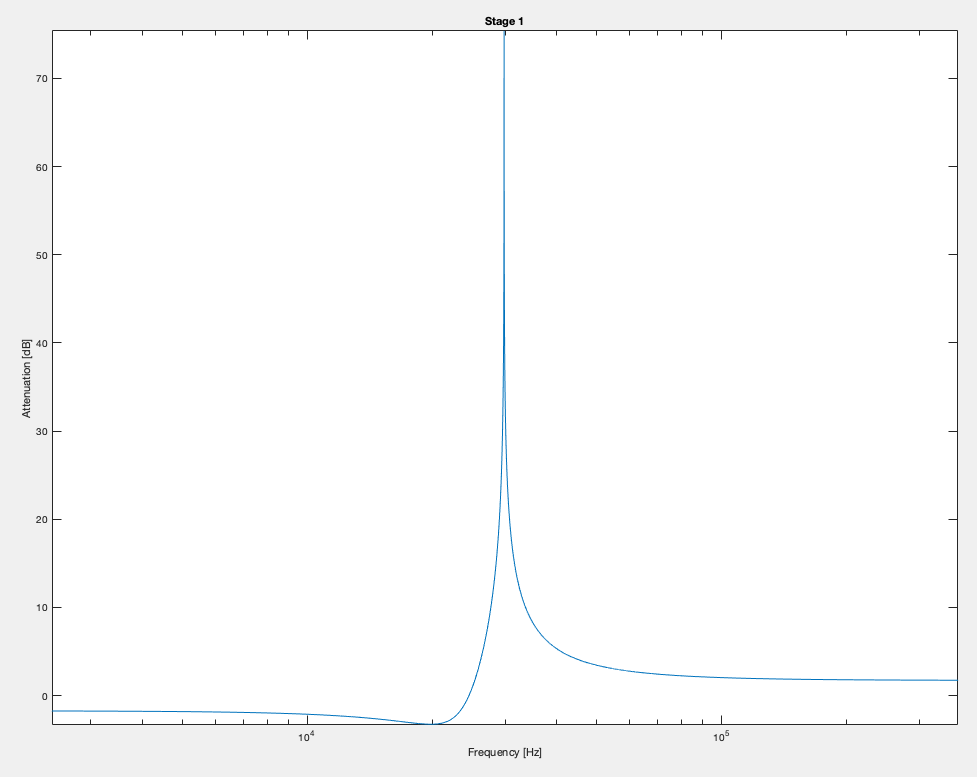
\includegraphics[width=.8\linewidth]{../Ex4/Resources/ej4_teorico_e1.png}  
      \caption{Etapa 1}
      \label{fig:ej4_bode_teorico_e1}
    \end{subfigure}
    \begin{subfigure}{.5\textwidth}
      \centering
      % include second image
      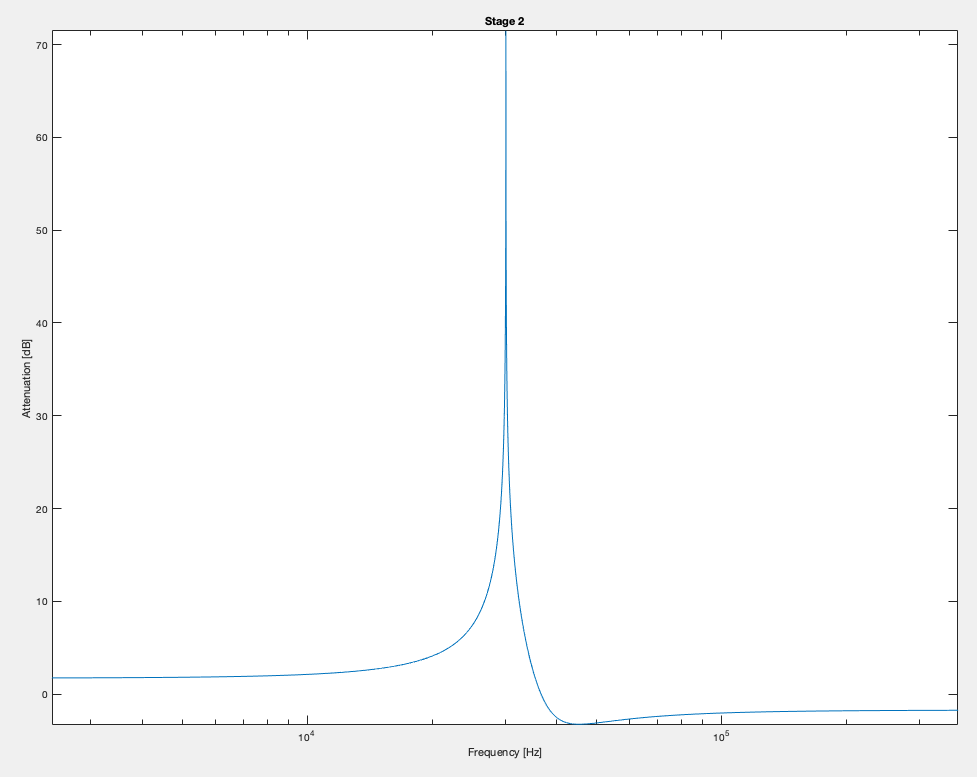
\includegraphics[width=.8\linewidth]{../Ex4/Resources/ej4_teorico_e2.png}  
      \caption{Etapa 2}
      \label{fig:sub-second}
    \end{subfigure}
    \caption{Atenuación de las etapas 1 y 2}
    \label{fig:ej4_bode_teorico_e2}
    \end{figure}


\begin{figure}[ht!]
    \centering
    \begin{subfigure}{.8\textwidth}
        \centering
        % include first image
        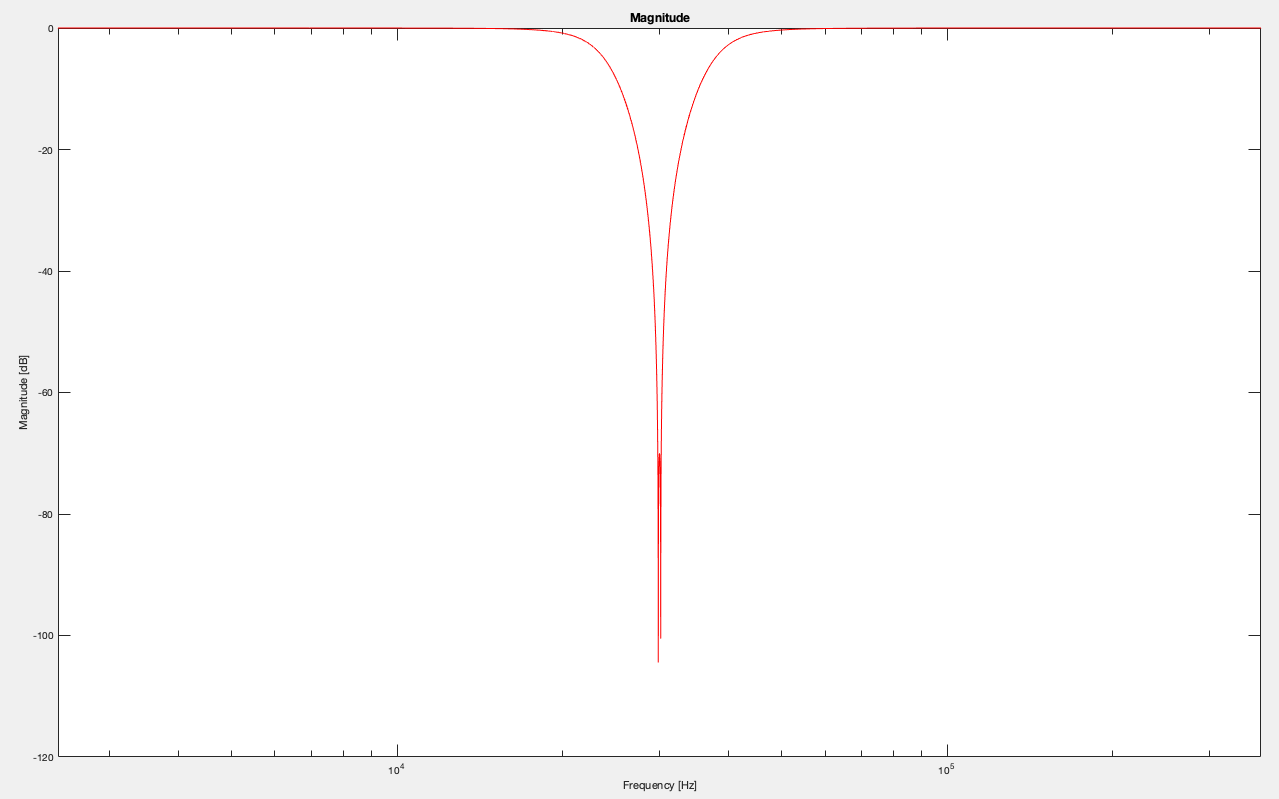
\includegraphics[width=.8\linewidth]{../Ex4/Resources/ej4_teorico_magnitud.png}  
        \caption{Magnitud}
    
    \end{subfigure}
    \begin{subfigure}{.8\textwidth}
        \centering
        % include second image
        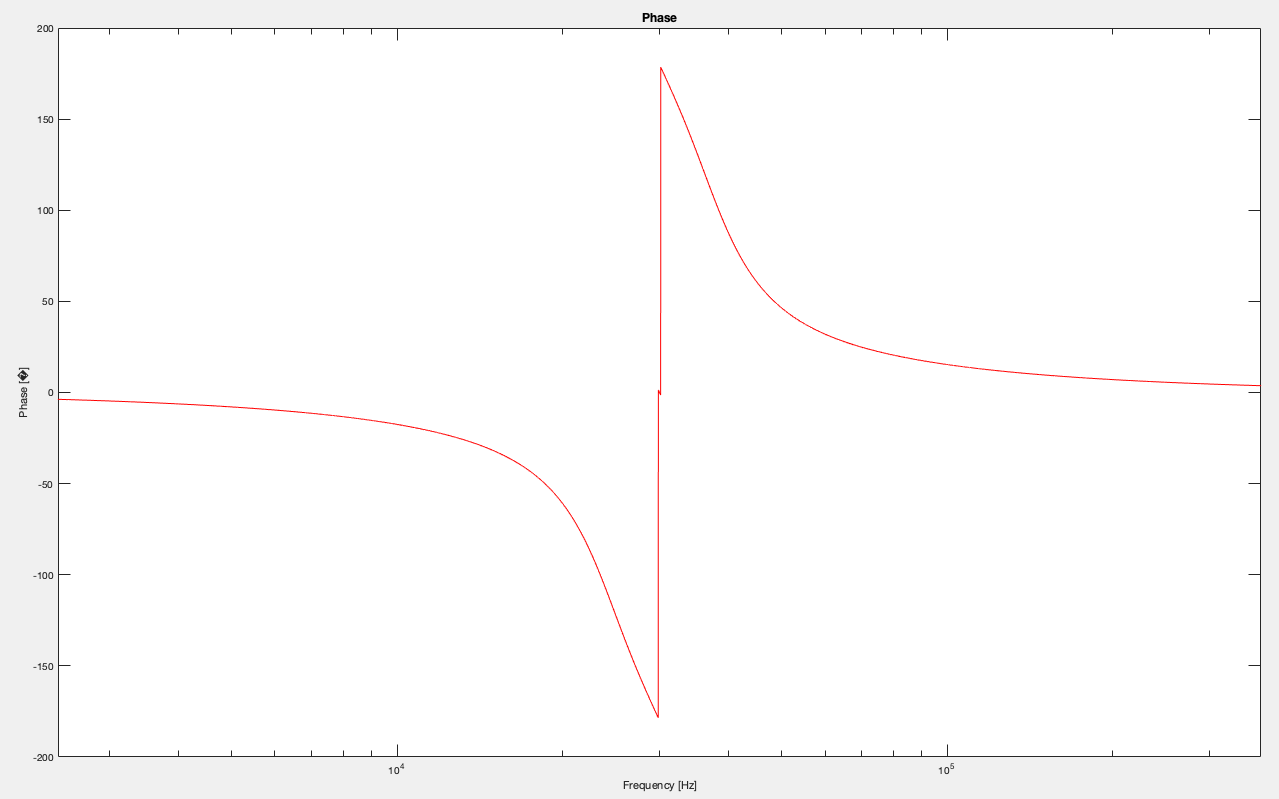
\includegraphics[width=.8\linewidth]{../Ex4/Resources/ej4_teorico_fase.png}  
        \caption{Fase}

    \end{subfigure}
    \caption{Bode del filtro calculado mediante el programa de aproximación}
    \label{fig:ej4_bode_teorico}
    \end{figure}





\section{Implementación}

En esta sección se analizan distintas configuraciones para luego poder diseñar la etapas del filtro. Recordar que, como se deben realizar dos etapas \textit{notch}, la celda debe estar configurada de modo que se pueda realizar la función trasferencia \ref{ej4_transferencia_notch}. En primer lugar se investiga sobre la celda universal \textit{Kerwin-Huelsman-Newcomb} creada por Kerwin, L. P. Huelsman y R. W. Newcomb en 1967 que utiliza dos integradores y un amplificador sumador. La celda se puede ver en la Figura \ref{fig:Kerwin-Huelsman-Newcomb}. La configuración provee una respuesta de segundo orden de pasa bajos, pasa banda y pasa altos. Es posible combinar estas respuestas para sintetizar una respuesta de \textit{notch} con la ayuda de un cuarto amplificador operacional. En esta configuración se puede demostrar que el factor de calidad $Q$ depende del ratio $\frac{R_2}{R_1}$. Luego, se tiene un $Q$ mucho mas sensible a las tolerancias de las resistencias, lo que es una desventaja. Una ventaja de esta celda es que cuenta con varias salidas para obtener las respuestas de pasa bajos, pasa banda y pasa altos (como se ve en la figura). Si se quiere obtener una respuesta \textit{notch}, como es le caso, se debe agregar un amplificador operacional mas que sume las salidas pasa alto y pasa bajo.

\begin{figure}[h!]                                                       
    \centering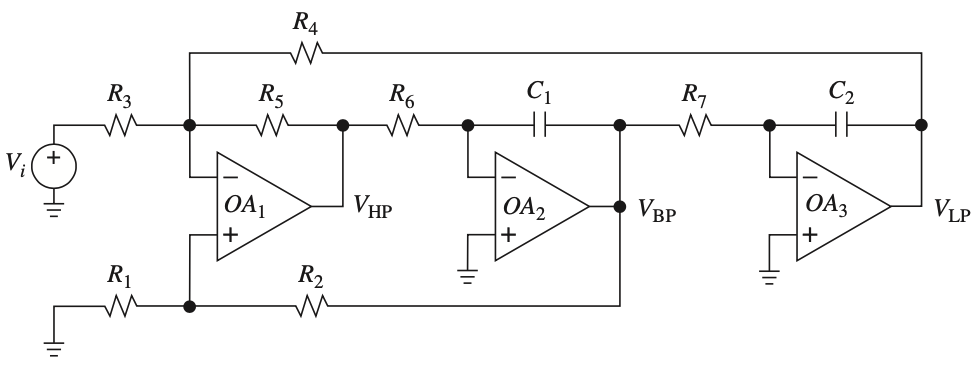
\includegraphics[width=0.9\textwidth]{../Ex4/Resources/Kerwin_Huelsman_Newcomb.png}
    \caption{Configuración Kerwin-Huelsman-Newcomb}
    \label{fig:Kerwin-Huelsman-Newcomb}
    \end{figure}

En segundo lugar, se investiga sobre la configuración \textit{Tow-Thomas}. La misma se puede ver en la Figura \ref{fig:Tow-Thomas}. La celda consiste en dos integradores, donde uno esta en configuración \textit{lossy} y un tercer amplificador operacional que tiene ganancia unitaria cuyo propósito es proveer inversión de polaridad. Se puede configurar uno de los integradores como no inversor, luego se puede eliminar el amplificador inversor dejando solo dos amplificadores operacionales. De todos modos esta configuración no provee la posibilidad de obtener ceros de trasmisión.   

\begin{figure}[h!]                                                       
    \centering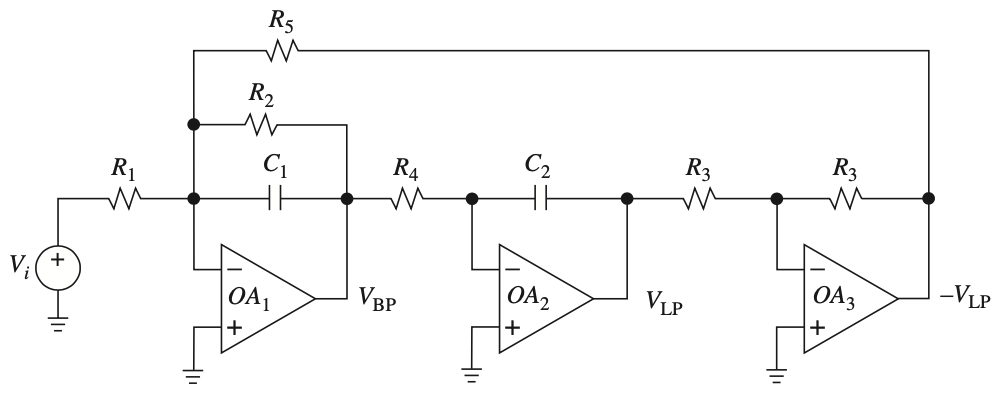
\includegraphics[width=0.9\textwidth]{../Ex4/Resources/Tow_Thomas.png}
    \caption{Configuración Tow-Thomas}
    \label{fig:Tow-Thomas}
    \end{figure}

En tercer lugar, se analiza la configuración \textit{Ackerberg-Mossberg} que esta basada en la configuración \textit{Tow-Thomas}. Lo que cambia entre ambas configuraciones es la implementación del integrador no inversor. Sin embargo, solamente  sirve para realizar filtros pasabanda y pasa bajos. Este circuito se ve muy limitado en muchas aplicaciones practicas que requieren ceros de transmisión en el plano $j\omega$. Es posible agregar ceros de transmisión mediante un sumador pero a costa de agregar un amplificador operacional lo que hace que el circuito tenga en total cuatro amplificadores operacionales. En la Figura \ref{fig:Ackerberg-Mossberg} se puede ver el circuito en configuración \textit{Ackerberg-Mossberg} que permitiría realizar la función transferencia \ref{ej4_transferencia_notch}. 

\begin{figure}[h!]                                                       
    \centering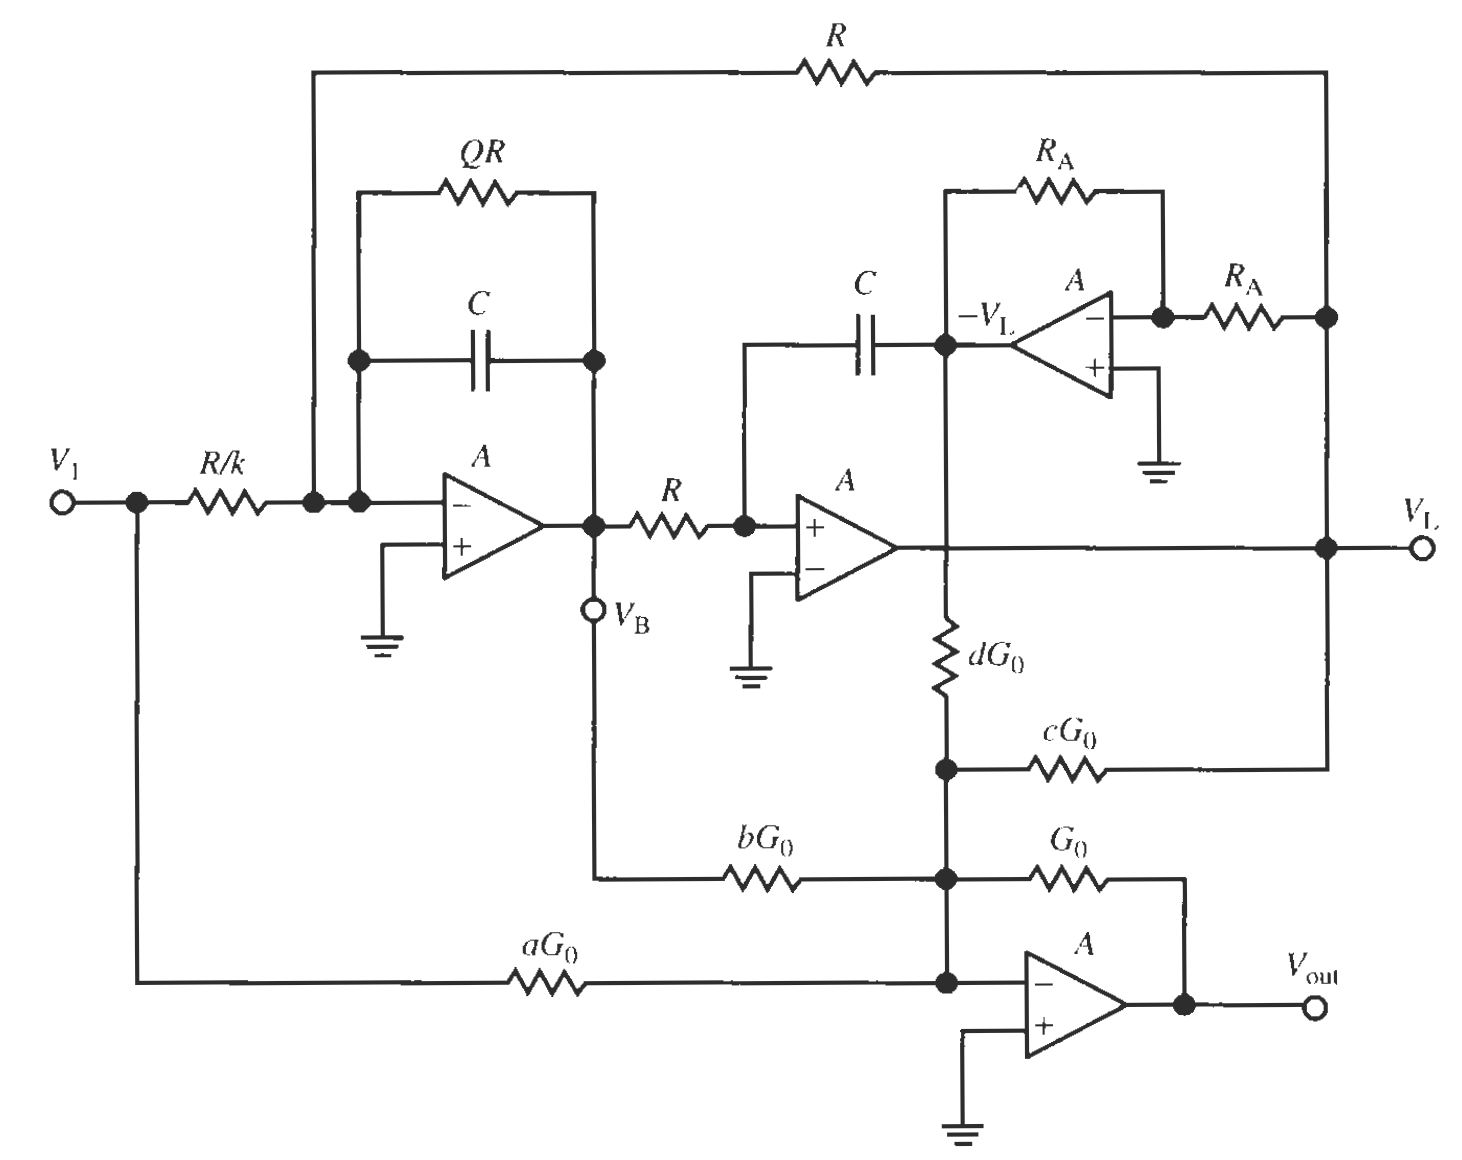
\includegraphics[width=0.9\textwidth]{../Ex4/Resources/Ackerberg_Mossberg.png}
    \caption{Configuración Ackerberg-Mossberg}
    \label{fig:Ackerberg-Mossberg}
    \end{figure}

Por ultimo, se analiza la celda \textit{Fleischer-Tow} que es otra modificación de la \textit{Tow-Thomas}. Esta celda cuenta con la ventaja que con tres amplificadores operacionales se puede obtener cualquier tipo de respuesta. En la Figura \ref{fig:celda_ft} se muestra la celda \textit{Fleischer-Tow}.


\begin{figure}[h!]                                                       
    \centering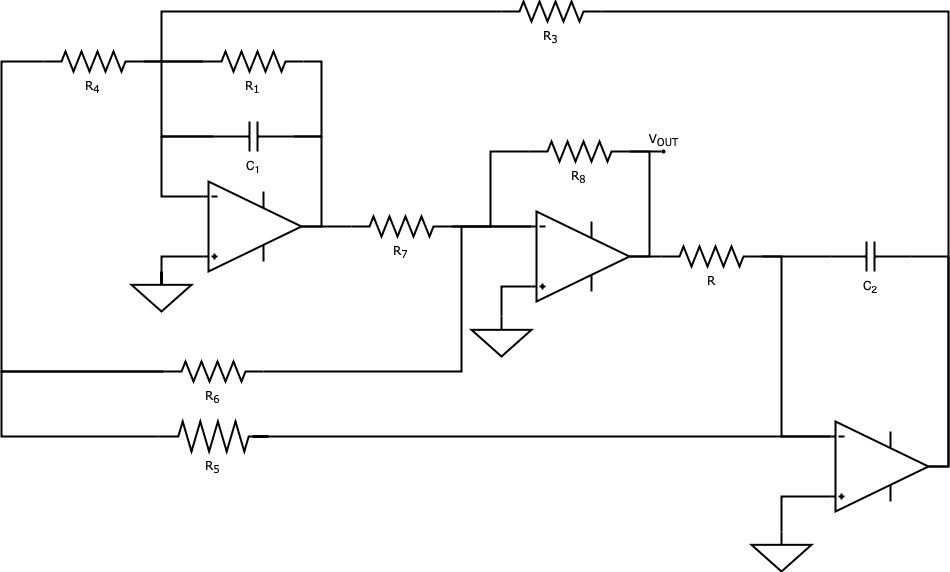
\includegraphics[width=0.9\textwidth]{../Ex4/Resources/ej4_FT.png}
    \caption{Configuración Fleischer-Tow}
    \label{fig:celda_ft}
    \end{figure}


\section{Diseño}

\subsection{Selección de configuracion de celda}
En la seccion anterior se mostraron las distintas configuraciones de celdas universales que se pueden utilizar. Como se vio, la celda \textit{Tow-Thomas} no permite obtener ceros de transmision por lo que se descarta para utilizarla. En cuanto a la \textit{Ackerberg-Mossberg} y la \textit{Kerwin-Huelsman-Newcomb}, si bien permiten obtener respuestas del tipo \textit{notch} requieren un amplificador mas. En consecuencia, como la celda \textit{Fleischer-Tow} solo requiere tres amplificadores operacionales para dar una respuesta \textit{notch} se opta por utilizar esta celda.  Como se mostró anteriormente, el circuito que describe dicha celda se puede ver en la Figura \ref{fig:celda_ft}. De dicho circuito es posible extraer la función transferencia. La misma se muestra a continuación:


\begin{equation} H(s) = - \frac{s^2 \frac{R_8}{R_6} + s \frac{R_8 (R_4 R_7 - R_1 R_6 )}{R_4 R_7 R_1 C_1} + \frac{R_8}{R_3 R_5 R_7 C_1 C_2}}{s^2 + s\frac{1}{R_1 C_1} + \frac{R_8}{R_2 R_3 R_7 C_1 C_2}} \label{ej4_ecu_funcion_transferencia_ft_completa}\end{equation} 

Se toman las siguientes igualdades para simplificar la función trasferencia y para que se asemeje lo mas posible a la función trasferencia de un filtro \textit{Notch} (\ref{ej4_transferencia_notch}) . Las mismas son:

\begin{displaymath}  R_4 = \frac{R_1 R_6}{R_7} \end{displaymath} 
\begin{displaymath}  C = C_1 = C_2  \end{displaymath} 
\begin{displaymath}  R_8 = R_7  \end{displaymath} 
\begin{displaymath}  R = R_2 = R_3  \end{displaymath} 
\begin{displaymath}  R_5 = R_6  \end{displaymath} 

La nueva función trasferencia resulta ser:

\begin{equation} H(s) = - \frac{s^2 \frac{R_8}{R_5} + \frac{1}{R_5 R C^2}}{s^2 + s\frac{1}{R_1 C_1} + \frac{1}{R_2 R_3 C^2}} \label{ej4_ecu_funcion_transferencia_ft}\end{equation}

Como se puede observar, (\ref{ej4_ecu_funcion_transferencia_ft}) tiene la forma de un filtro \textit{Notch}. Solo resta obtener las relaciones de los parámetros del filtro ($\omega_p$, $\omega_z$ y $Q$) con los componentes de la celda. Nuevamente se utiliza la función trasferencia (\ref{ej4_transferencia_notch}) para extraer dichas relaciones:

\begin{displaymath}  R = \frac{1}{\omega_p C}  \end{displaymath} 
\begin{displaymath}  R_1 = \frac{Q}{\omega_p C}  \end{displaymath} 
\begin{displaymath}  R_5 = \frac{1}{k \omega^2_z R C^2}  \end{displaymath} 
\begin{displaymath}  R_8 = k R_5 \end{displaymath} 

Para simplificar las cuentas y como no hay posibilidad de saturar a los amplificadores operacionales involucrados, se define $k=1$.  Nótese, que que solamente hay tres valores de resistencia diferentes. Esto se puede ver como una ventaja ya que disminuye la complejidad del circuito. Ya es posible armar una celda con configuración \textit{Fleischer-Tow} que describe un filtro \textit{Notch}. La misma se puede ver en la Figura \ref{ej4_circuito_ft_notch}. Como ya es sabido la configuración \textit{Fleischer-Tow} cuenta con tres amplificadores por lo que se decide utilizar el integrado TL084 ya que contiene cuatro amplificadores operacionales. 

\begin{figure}[h!]                                                       
    \centering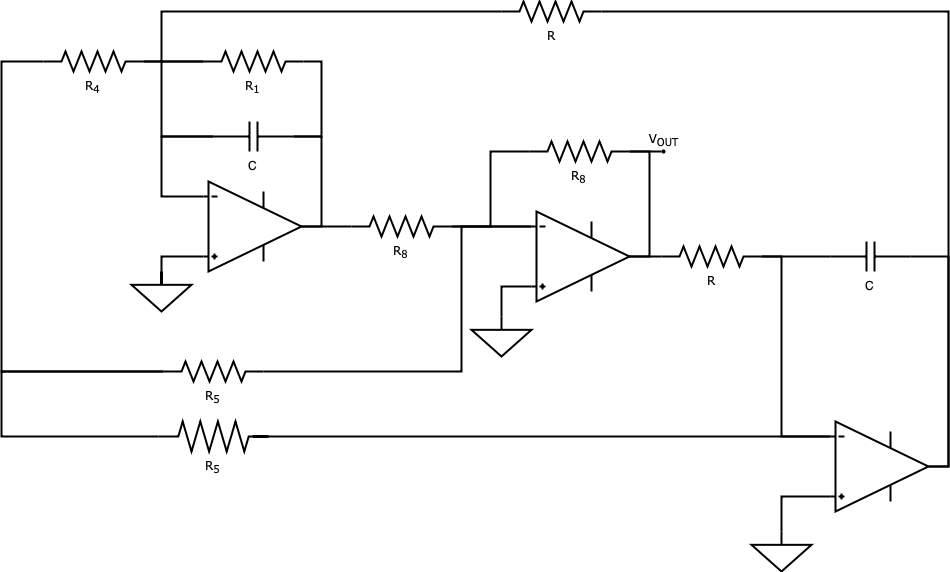
\includegraphics[width=0.8\textwidth]{../Ex4/Resources/FT_notch.png}
    \caption{Filtro \textit{Notch} implementado con \textit{Fleischer-Tow}}
    \label{ej4_circuito_ft_notch}
    \end{figure}

\subsection{Selección de componentes}
Al tener el circuito que describe un filtro \textit{Notch} es posible continuar con el diseño del filtro deseado. Como se vio anteriormente, para cumplir la plantilla se requieren dos etapas. La primera etapa tiene $Q = 2.54$ y contiene el siguiente polo y cero:

\begin{displaymath}  f_{p1}   = 24479 Hz\end{displaymath} 
\begin{displaymath}  f_{z1}   = 29848 Hz\end{displaymath} 

Gracias a estos valores y a las relaciones anteriormente calculadas, se pueden calcular los valores de los componentes. Los resultados se muestran en la Tabla \ref{tab:ej4_e1_componentes_calculados}.

\begin{table}[h!]
    \centering
    \begin{tabular}{|c|c|}
    \hline
    $R_1$ & $16514 \Omega$ \\ \hline
    $R$   & $6501\Omega$   \\ \hline
    $R_5$ & $4373 \Omega$  \\ \hline
    $R_4$ & $16514 \Omega$ \\ \hline

    $R_8$ & $4373 \Omega$ \\ \hline
    \end{tabular}
    \caption{Componentes calculados etapa 1}
    \label{tab:ej4_e1_componentes_calculados}
    \end{table}

Como los valores de la Tabla \ref{tab:ej4_e1_componentes_calculados} no son comerciales, se utilizan los que se muestran en la Tabla \ref{tab:ej4_e1_componentes}.

\begin{table}[h!]
    \centering
    \begin{tabular}{|c|c|}
    \hline
    $R_1$ & $33k\Omega // 33k\Omega$ \\ \hline
    $R$   & $6.2k$   \\ \hline
    $R_5$ & $4.3k \Omega$  \\ \hline
    $R_4$ & $33k\Omega // 33k\Omega$ \\ \hline
    $R_8$ & $4.3k \Omega$ \\ \hline
    \end{tabular}
    \caption{Componentes comerciales etapa 1}
    \label{tab:ej4_e1_componentes}
    \end{table}


Por otro lado, la segunda etapa tiene un $Q = 2.54$ y contiene el siguiente polo y cero en:

\begin{displaymath}  f_{p2}   = 36764 Hz\end{displaymath} 
\begin{displaymath}  f_{z2}   = 30151 Hz\end{displaymath} 

Los valores de los componentes se muestran en la Tabla \ref{tab:ej4_e2_componentes_calculados} y en la Tabla \ref{tab:ej4_e2_componentes} se muestran los valores comerciales.

\begin{table}[h!]
    \centering
    \begin{tabular}{|c|c|}
    \hline
    $R_1$ & $ 10995 \Omega$ \\ \hline
    $R$   & $4329\Omega$   \\ \hline
    $R_5$ & $6436 \Omega$  \\ \hline
    $R_4$ & $10995 \Omega$ \\ \hline
    $R_8$ & $6436 \Omega$ \\ \hline
    \end{tabular}
    \caption{Componentes calculados etapa 2}
    \label{tab:ej4_e2_componentes_calculados}
    \end{table} 


\begin{table}[h!]
    \centering
    \begin{tabular}{|c|c|}
    \hline
    $R_1$ & $11k\Omega$ \\ \hline
    $R$   & $4.3k$   \\ \hline
    $R_5$ & $6.2k \Omega$  \\ \hline
    $R_4$ & $11k \Omega$ \\ \hline
    $R_8$ & $6.2k \Omega$ \\ \hline
    \end{tabular}
    \caption{Componentes comerciales etapa 2}
    \label{tab:ej4_e2_componentes}
    \end{table}

Cabe aclarar que para ambas etapas se utiliza $C = 1nF$ ya que con dicho valor las resistencias adquieren valores del orden de los $k\Omega$. 

Si ambas etapas se ponen en cascada y se simula, se obtiene el bode de la Figura \ref{ej4_simulacion_comerciales}. En primer lugar, se puede destacar que se cumple la profundidad del notch, lo que es satisfactorio. Sin embargo, la frecuencia en la que se produce el notch no es exactamente $30kHz$ si se utilizan los valores de los componentes de los componentes propuestos. Esto se debe principalmente a que los valores necesarios para que se de en esta frecuencia no existen comercialmente. Al aproximar los valores de las resistencias se produce este error. Para solucionar este problema se decide utilizar un preset en ambas etapas en el lugar de $R_7$. Como se vera mas adelante, la sensibilidad de $R_7$ implica una modificación en la ubicación de los ceros en ambas etapas. Luego, se explota esta situación para calibrar el circuito de manera que ambas etapas tengan los ceros donde corresponde y que al tener las etapas en cascada la frecuencia se ubique en $30kHz$. Luego, al tener esta nueva opción, se encontró que si $R_7$ es $4100 \Omega$ para la primera etapa y $6300 \Omega$ para la segunda etapa la simulación cumple con la plantilla del filtro. La Figura \ref{ej4_simulacion_comerciales} muestra el bode del filtro con estas modificaciones. Habiendo aclarado esto, se cambia $R_7$ de la primera etapa por un preset de $5k \Omega$ y por uno de $10k \Omega$ para la segunda etapa. 

\begin{figure}[h!]                                                       
    \centering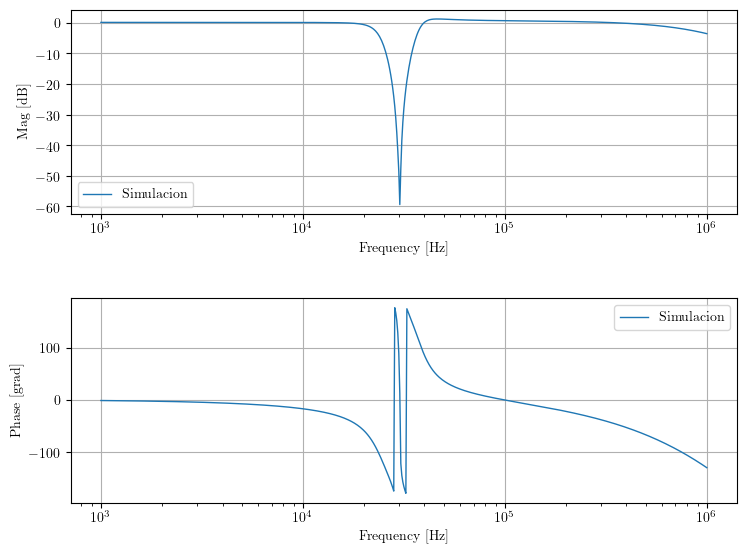
\includegraphics[width=0.9\textwidth]{../Ex4/Resources/ej4_bode_sim.png}
    \caption{Simulación del filtro con componentes comerciales}
    \label{ej4_simulacion_comerciales}
    \end{figure}


\subsection{Sensibilidades}

En esta sección se busca analizar la sensibilidad de los componentes del circuito propuesto. Para calcular las sensibilidades se utiliza la siguiente ecuación:

\begin{displaymath}  S^{g(x)}_{x_k} = \frac{\delta g(x)} {\delta x_k} \frac{x_k}{g(x)}\end{displaymath}
    
En primer lugar, se calcula la sensibilidad de $Q_z$. Recordando la función trasferencia completa de la celda \textit{Fleischer-Tow} (\ref{ej4_ecu_funcion_transferencia_ft_completa}) se extrae la expresión del factor de calidad de cero $Q_z$:

\begin{displaymath} Q_z = \frac{R_4 R_7 C_1 \omega_z}{R_8 (R_4 R_7 - R_1 R_6)} = \frac{R_1 R_4}{R_4 R_7 - R_1 R_6} \sqrt{\frac{C_1 R_8 R_7}{R_3 R_5 C_2}}\end{displaymath}

Gracias a un algoritmo, se obtienen los siguientes resultados:

\begin{displaymath}  S^{Q_z}_{R_1} = \frac{R_4 R_7} {R_1 R_6 - R_4 R_7}\end{displaymath}
\begin{displaymath}  S^{Q_z}_{R_3} = \frac{-1} {2}\end{displaymath}
\begin{displaymath}  S^{Q_z}_{R_4} = \frac{R_1 R_6} {R_1 R_6 - R_4 R_7}\end{displaymath}
\begin{displaymath}  S^{Q_z}_{R_5} = \frac{-1} {2}\end{displaymath}
\begin{displaymath}  S^{Q_z}_{R_6} = -\frac{R_1 R_6 + R_4 R_7} {2(R_1 R_6 - R_4 R_7)}\end{displaymath}
\begin{displaymath}  S^{Q_z}_{R_7} = \frac{R_1 R_6 + R_4 R_7} {2(R_1 R_6 - R_4 R_7)}\end{displaymath}
\begin{displaymath}  S^{Q_z}_{C_1} = \frac{1} {2}\end{displaymath}
\begin{displaymath}  S^{Q_z}_{C_2} = \frac{-1} {2}\end{displaymath}

En segundo lugar, se calcula la sensibilidad de $Q$. La expresión de $Q$ es:

\begin{displaymath} Q_ = \sqrt{\frac{R_8 C_1 }{R_2 R_3 R_7 C_2}} R_1\end{displaymath}

Gracias a un algoritmo, se obtienen los siguientes resultados:
\begin{displaymath}  S^{Q}_{R_1} = 1\end{displaymath}
\begin{displaymath}  S^{Q}_{R_2} = -\frac{1}{2}\end{displaymath}
\begin{displaymath}  S^{Q}_{R_3} = -\frac{1}{2}\end{displaymath}
\begin{displaymath}  S^{Q}_{R_7} = -\frac{1}{2}\end{displaymath}
\begin{displaymath}  S^{Q}_{R_8} = \frac{1}{2}\end{displaymath}
\begin{displaymath}  S^{Q}_{C_1} = \frac{1}{2}\end{displaymath}
\begin{displaymath}  S^{Q}_{R_2} = -\frac{1}{2}\end{displaymath}

En tercer lugar, se calcula la sensibilidad de $\omega_0$. Se recuerda su expresión:
\begin{displaymath}  \omega_0 = \sqrt{\frac{R_8}{R_2 R_3 R_7 C_1 C_2}}\end{displaymath}

Gracias a un algoritmo, se obtienen los siguientes resultados:
\begin{displaymath}  S^{\omega_0}_{R_2} = -\frac{1}{2}\end{displaymath}
\begin{displaymath}  S^{\omega_0}_{R_3} = -\frac{1}{2}\end{displaymath}
\begin{displaymath}  S^{\omega_0}_{R_7} = -\frac{1}{2}\end{displaymath}
\begin{displaymath}  S^{\omega_0}_{R_8} = \frac{1}{2}\end{displaymath}
\begin{displaymath}  S^{\omega_0}_{C_1} = -\frac{1}{2}\end{displaymath}
\begin{displaymath}  S^{\omega_0}_{C_2} = -\frac{1}{2}\end{displaymath}

En cuarto lugar, se calcula la sensibilidad de $\omega_z$. Se recuerda su expresión:

\begin{displaymath}  \omega_z = \sqrt{\frac{R_8}{R_3 R_5 R_7 C_1 C_2}}\end{displaymath}

Gracias a un algoritmo, se obtienen los siguientes resultados:

\begin{displaymath}  S^{\omega_z}_{R_3} = -\frac{1}{2}\end{displaymath}
\begin{displaymath}  S^{\omega_z}_{R_5} = -\frac{1}{2}\end{displaymath}
\begin{displaymath}  S^{\omega_z}_{R_7} = -\frac{1}{2}\end{displaymath}
\begin{displaymath}  S^{\omega_z}_{R_8} = \frac{1}{2}\end{displaymath}
\begin{displaymath}  S^{\omega_z}_{C_1} = -\frac{1}{2}\end{displaymath}
\begin{displaymath}  S^{\omega_z}_{C_2} = -\frac{1}{2}\end{displaymath}

Por ultimo se calcula la sensibilidad de $G$. La expresión de $G$ es:

\begin{displaymath}  G = \frac{R_8}{R_6}\end{displaymath}
Se puede ver fácilmente que:
    
\begin{displaymath}  S^{G}_{R_8} = 1\end{displaymath}
\begin{displaymath}  S^{G}_{R_6} = -1\end{displaymath}


\subsection{Análisis de montecarlo}

Es de importancia aclarar que, para implementar el circuito, se utilizan todas resistencias SMD ya que tienen tolerancia de aproximadamente $1\%$. La Figura \ref{ej4_montecarlo} muestra el análisis de montecarlo sobre el circuito. Como se puede observar, tanto la profundidad del notch como la frecuencia a la que este se ubica varían considerablemente. Esto provoca que la plantilla no se cumpla en varios casos. Como se vio en la sección de sensibilidad, la mayoría de los componentes afectan considerablemente el comportamiento del circuito, a pesar de utilizar resistencias baja tolerancia. Para solucionar este problema, se vuelve a recurrir a la opción del preset en la resistencia $R_7$. El preset en ambas etapas calibra el circuito para que los ceros se ubiquen donde corresponden compensando las variaciones de los componentes. 


\begin{figure}[ht!]
    \centering
    \begin{subfigure}{.8\textwidth}
        \centering
        % include first image
        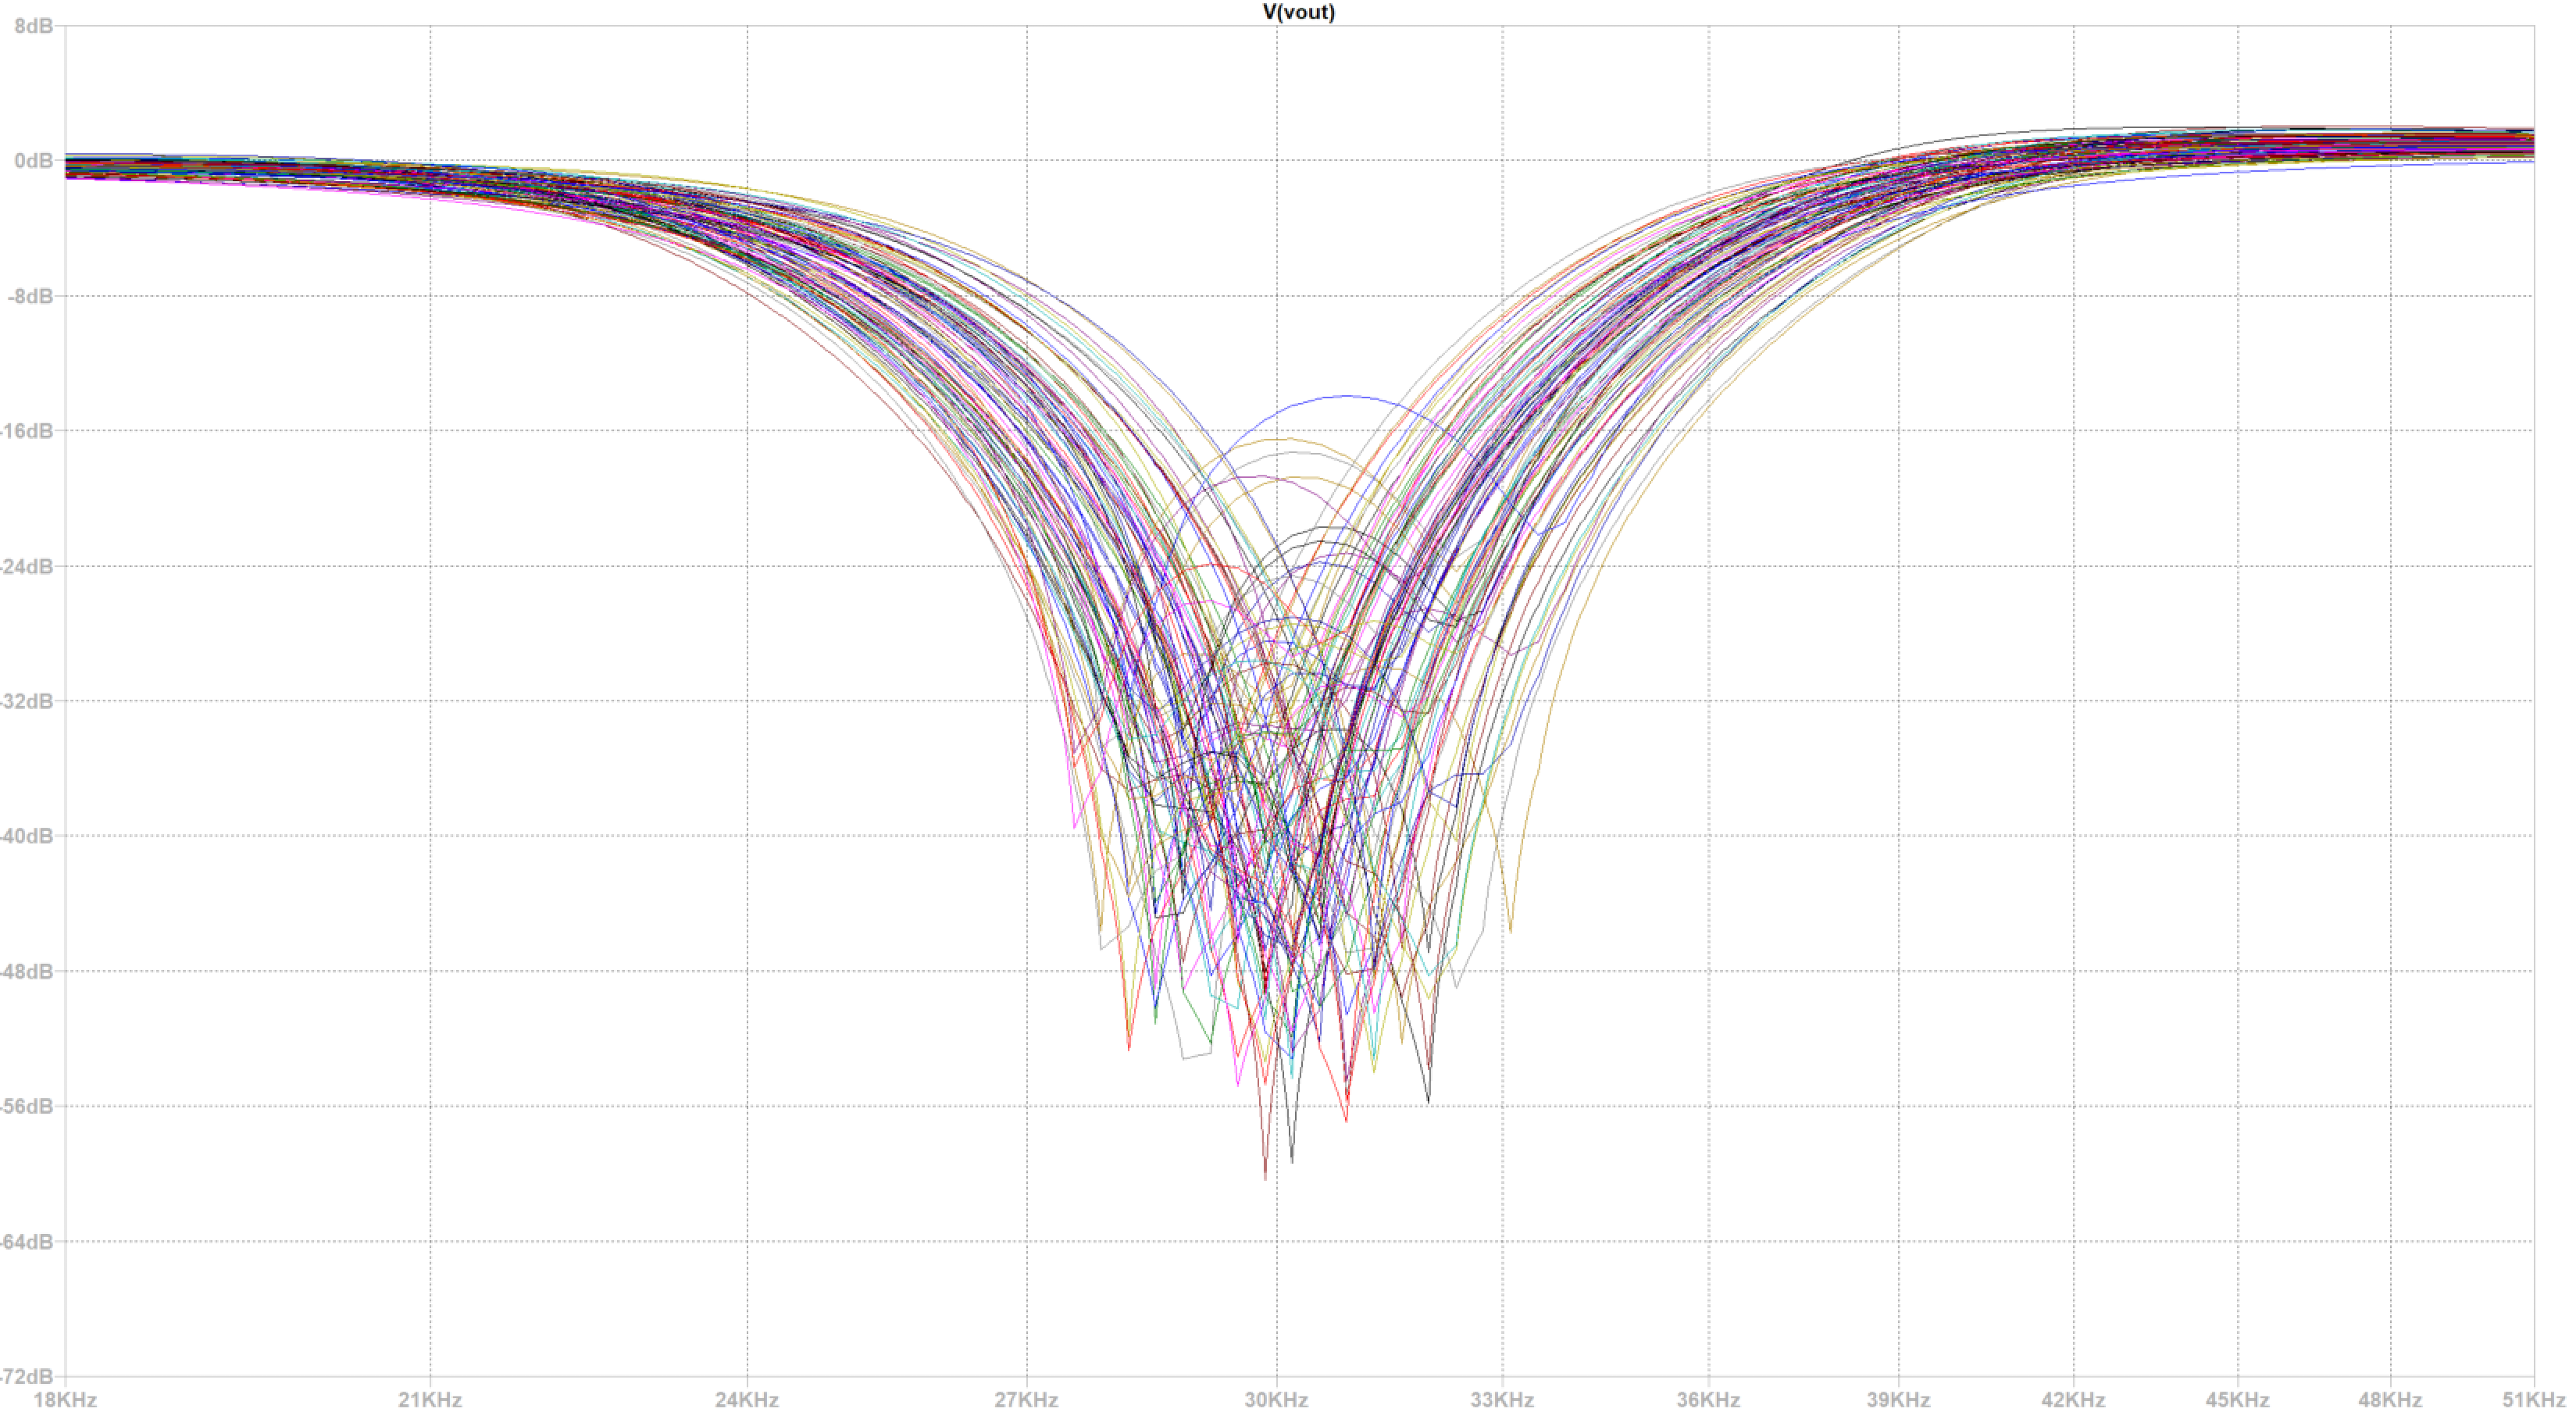
\includegraphics[width=.9\linewidth]{../Ex4/Resources/ej4_montecarlo_mag.png}  
        \caption{Magnitud}
    
    \end{subfigure}
    \begin{subfigure}{.8\textwidth}
        \centering
        % include second image
        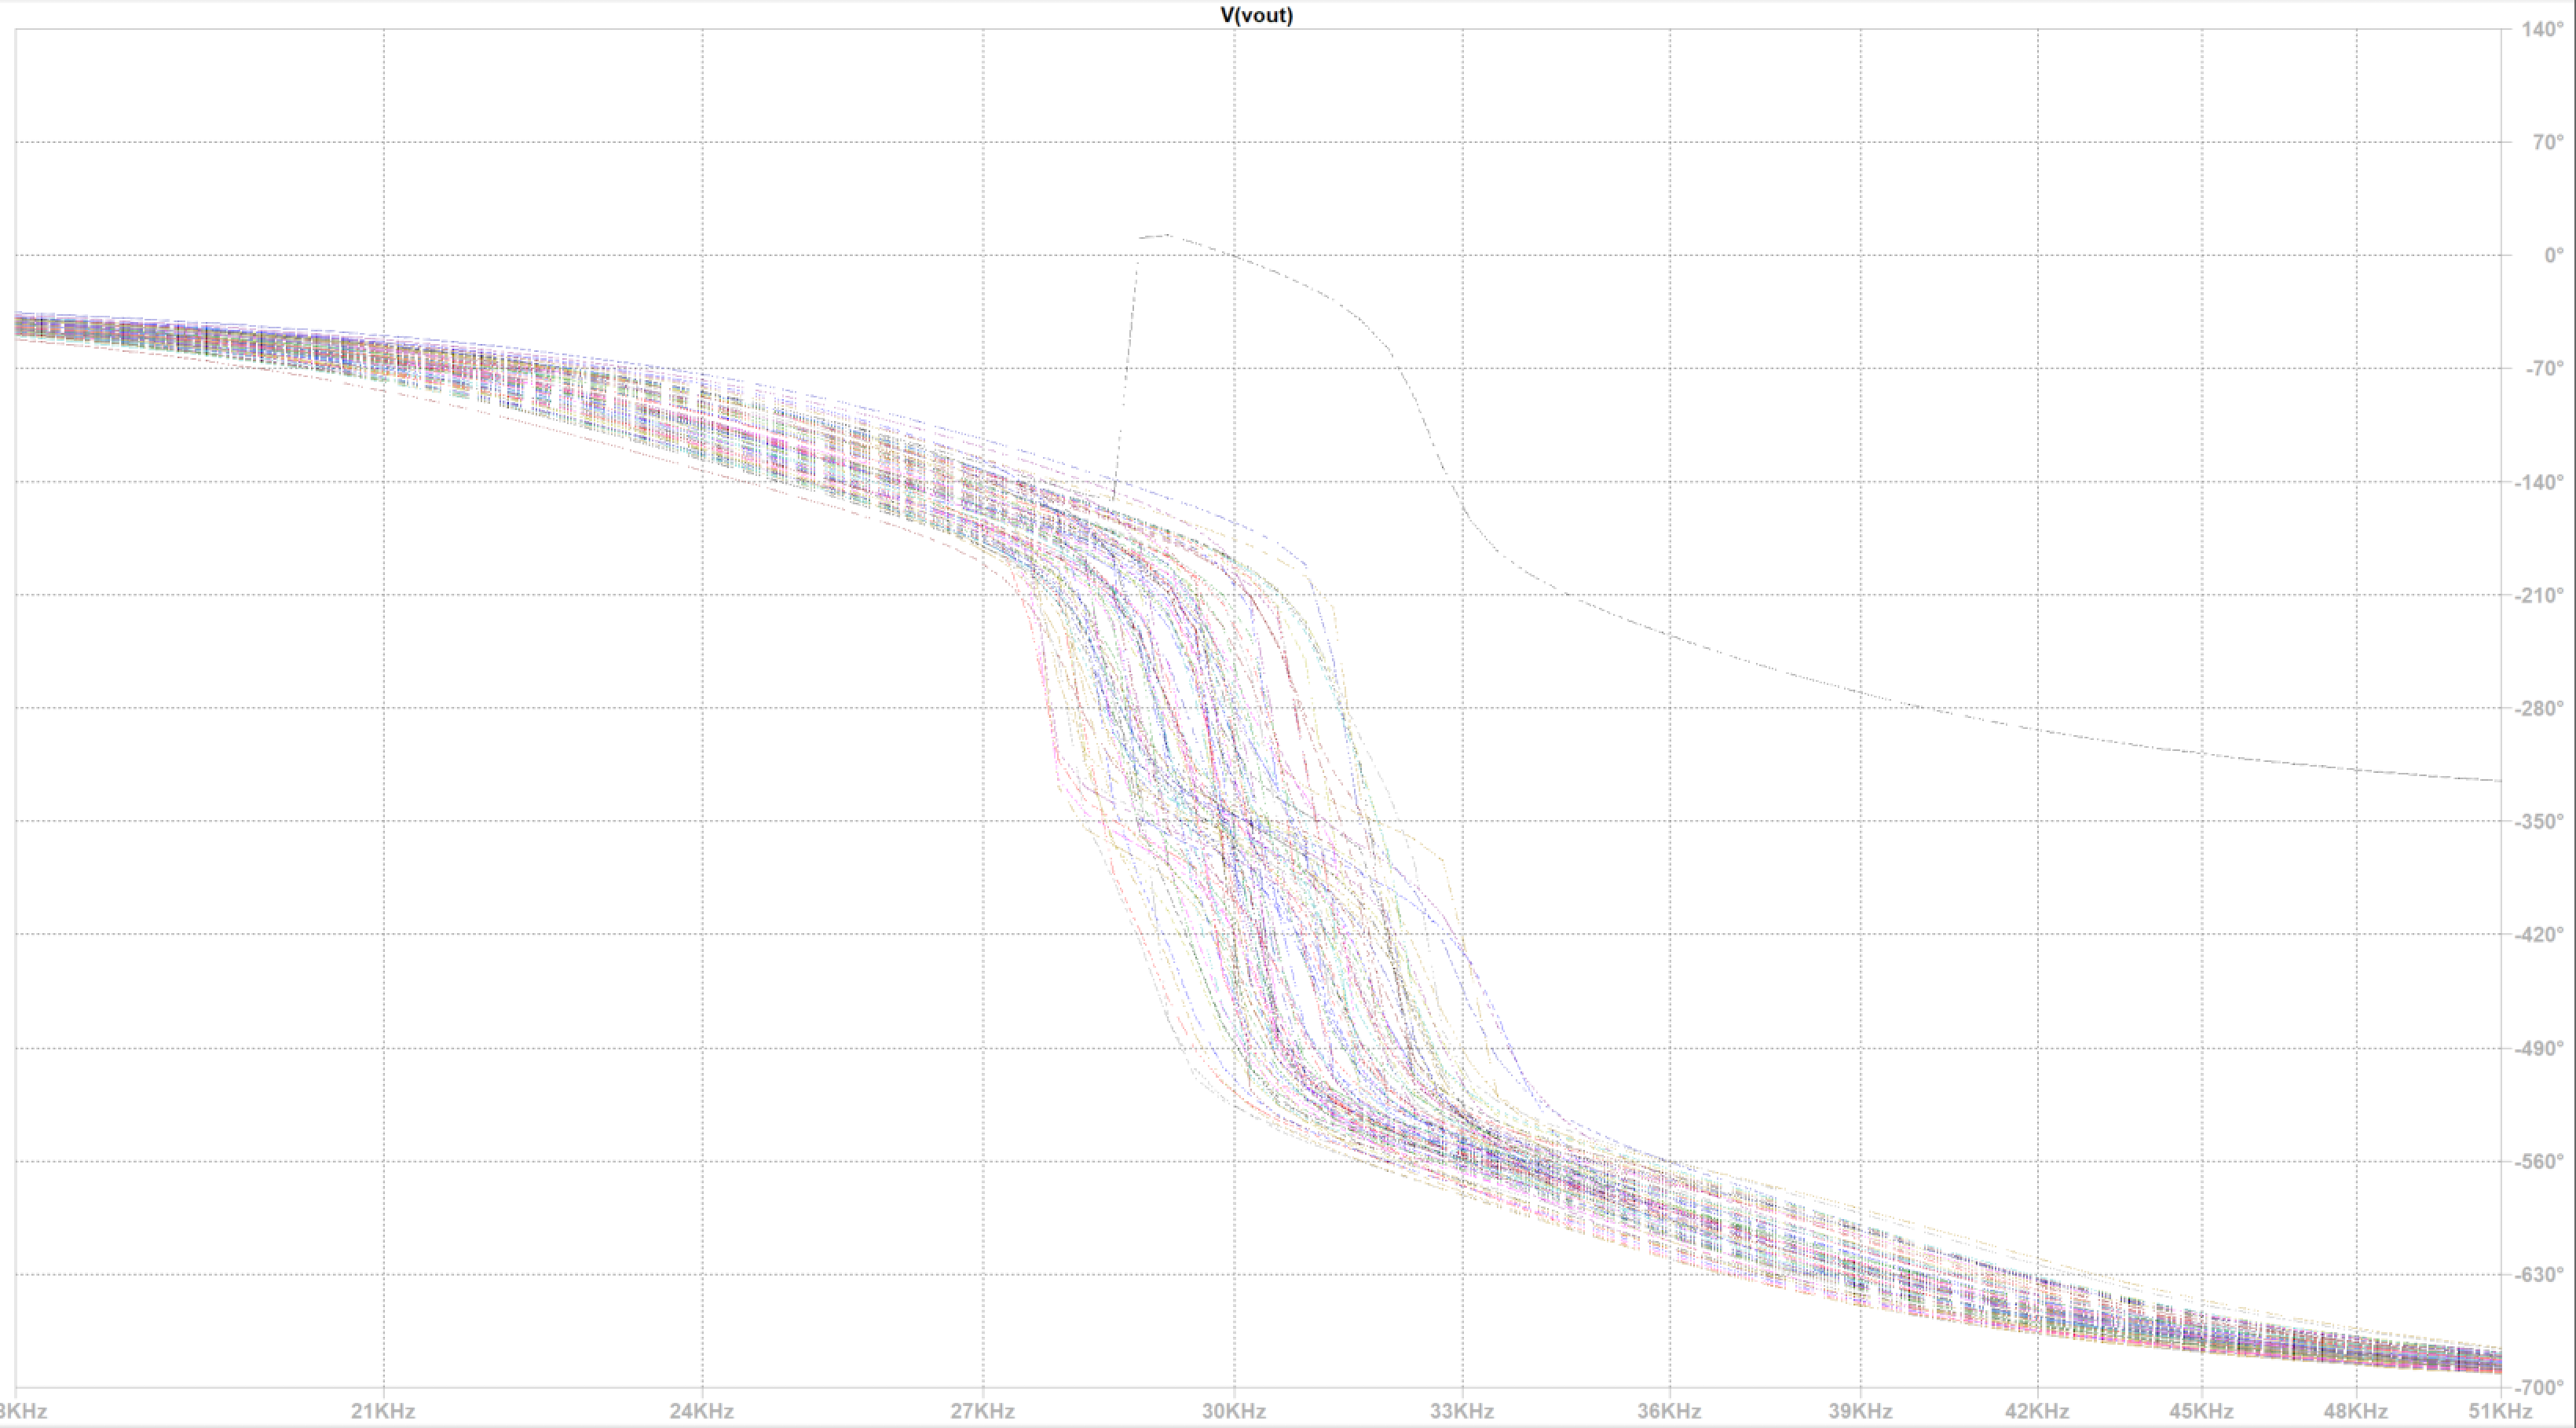
\includegraphics[width=.9\linewidth]{../Ex4/Resources/ej4_montecarlo_fase.png}  
        \caption{Fase}

    \end{subfigure}
    \caption{Análisis montecarlo}
    \label{ej4_montecarlo}
    \end{figure}
    


\subsection{Impedancia de entrada}

Como la plantilla impone  que la impedancia de entrada sea mayor a $50k \Omega$ se decide incorporar buffers a la entrada de ambas etapas. Como cada etapa del circuito es implementada con dos integrados TL084 que contiene cuatro operacionales, es posible utilizar uno de ellos como buffer. Con esta configuración, la simulación de la impedancia de entrada se puede ver en la Figura \ref{ej4_simulacion_impedancia_entrada}. Como se puede observar, con esta configuración se cumple ampliamente la condición de la impedancia de entrada. 

\begin{figure}[h!]                                                
    \centering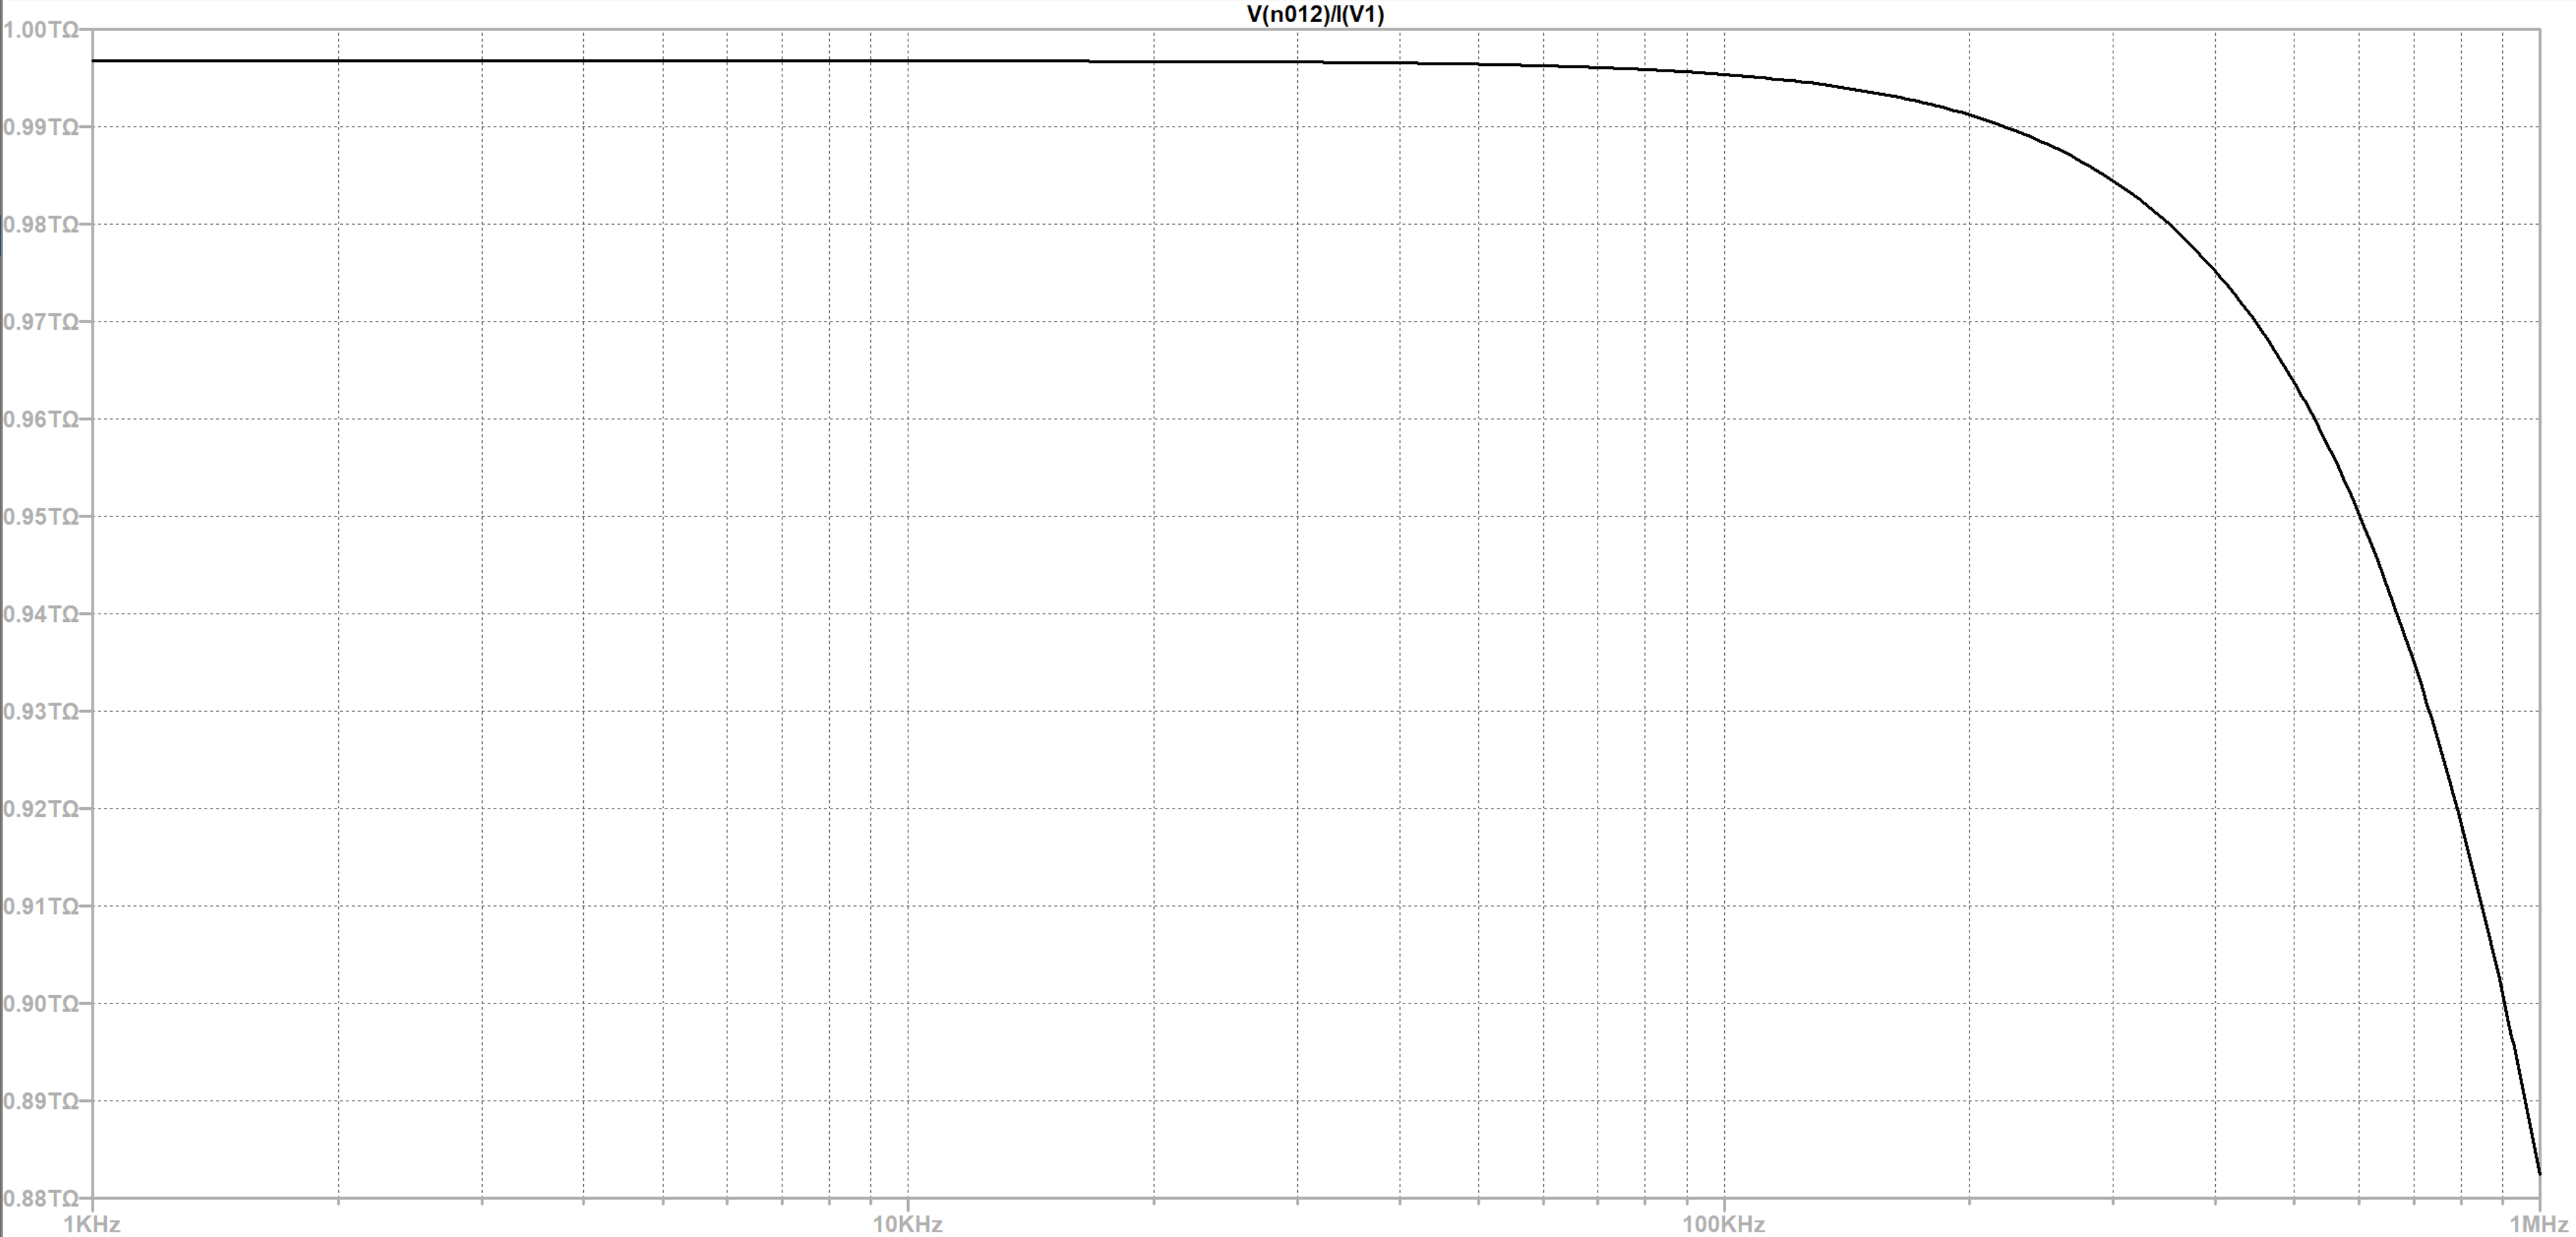
\includegraphics[width=0.9\textwidth]{../Ex4/Resources/ej4_impedancia.png}
    \caption{Simulación de impedancia de entrada}
    \label{ej4_simulacion_impedancia_entrada}
    \end{figure}



\subsection{Impedancia de salida}
En la Figura \ref{fig:ej4_impedancia_salida} se puede ver la simulación de la impedancia de salida. Como se puede ver, aumenta abruptamente a a partir de $100kHz$. 

\begin{figure}[h!]                                                
    \centering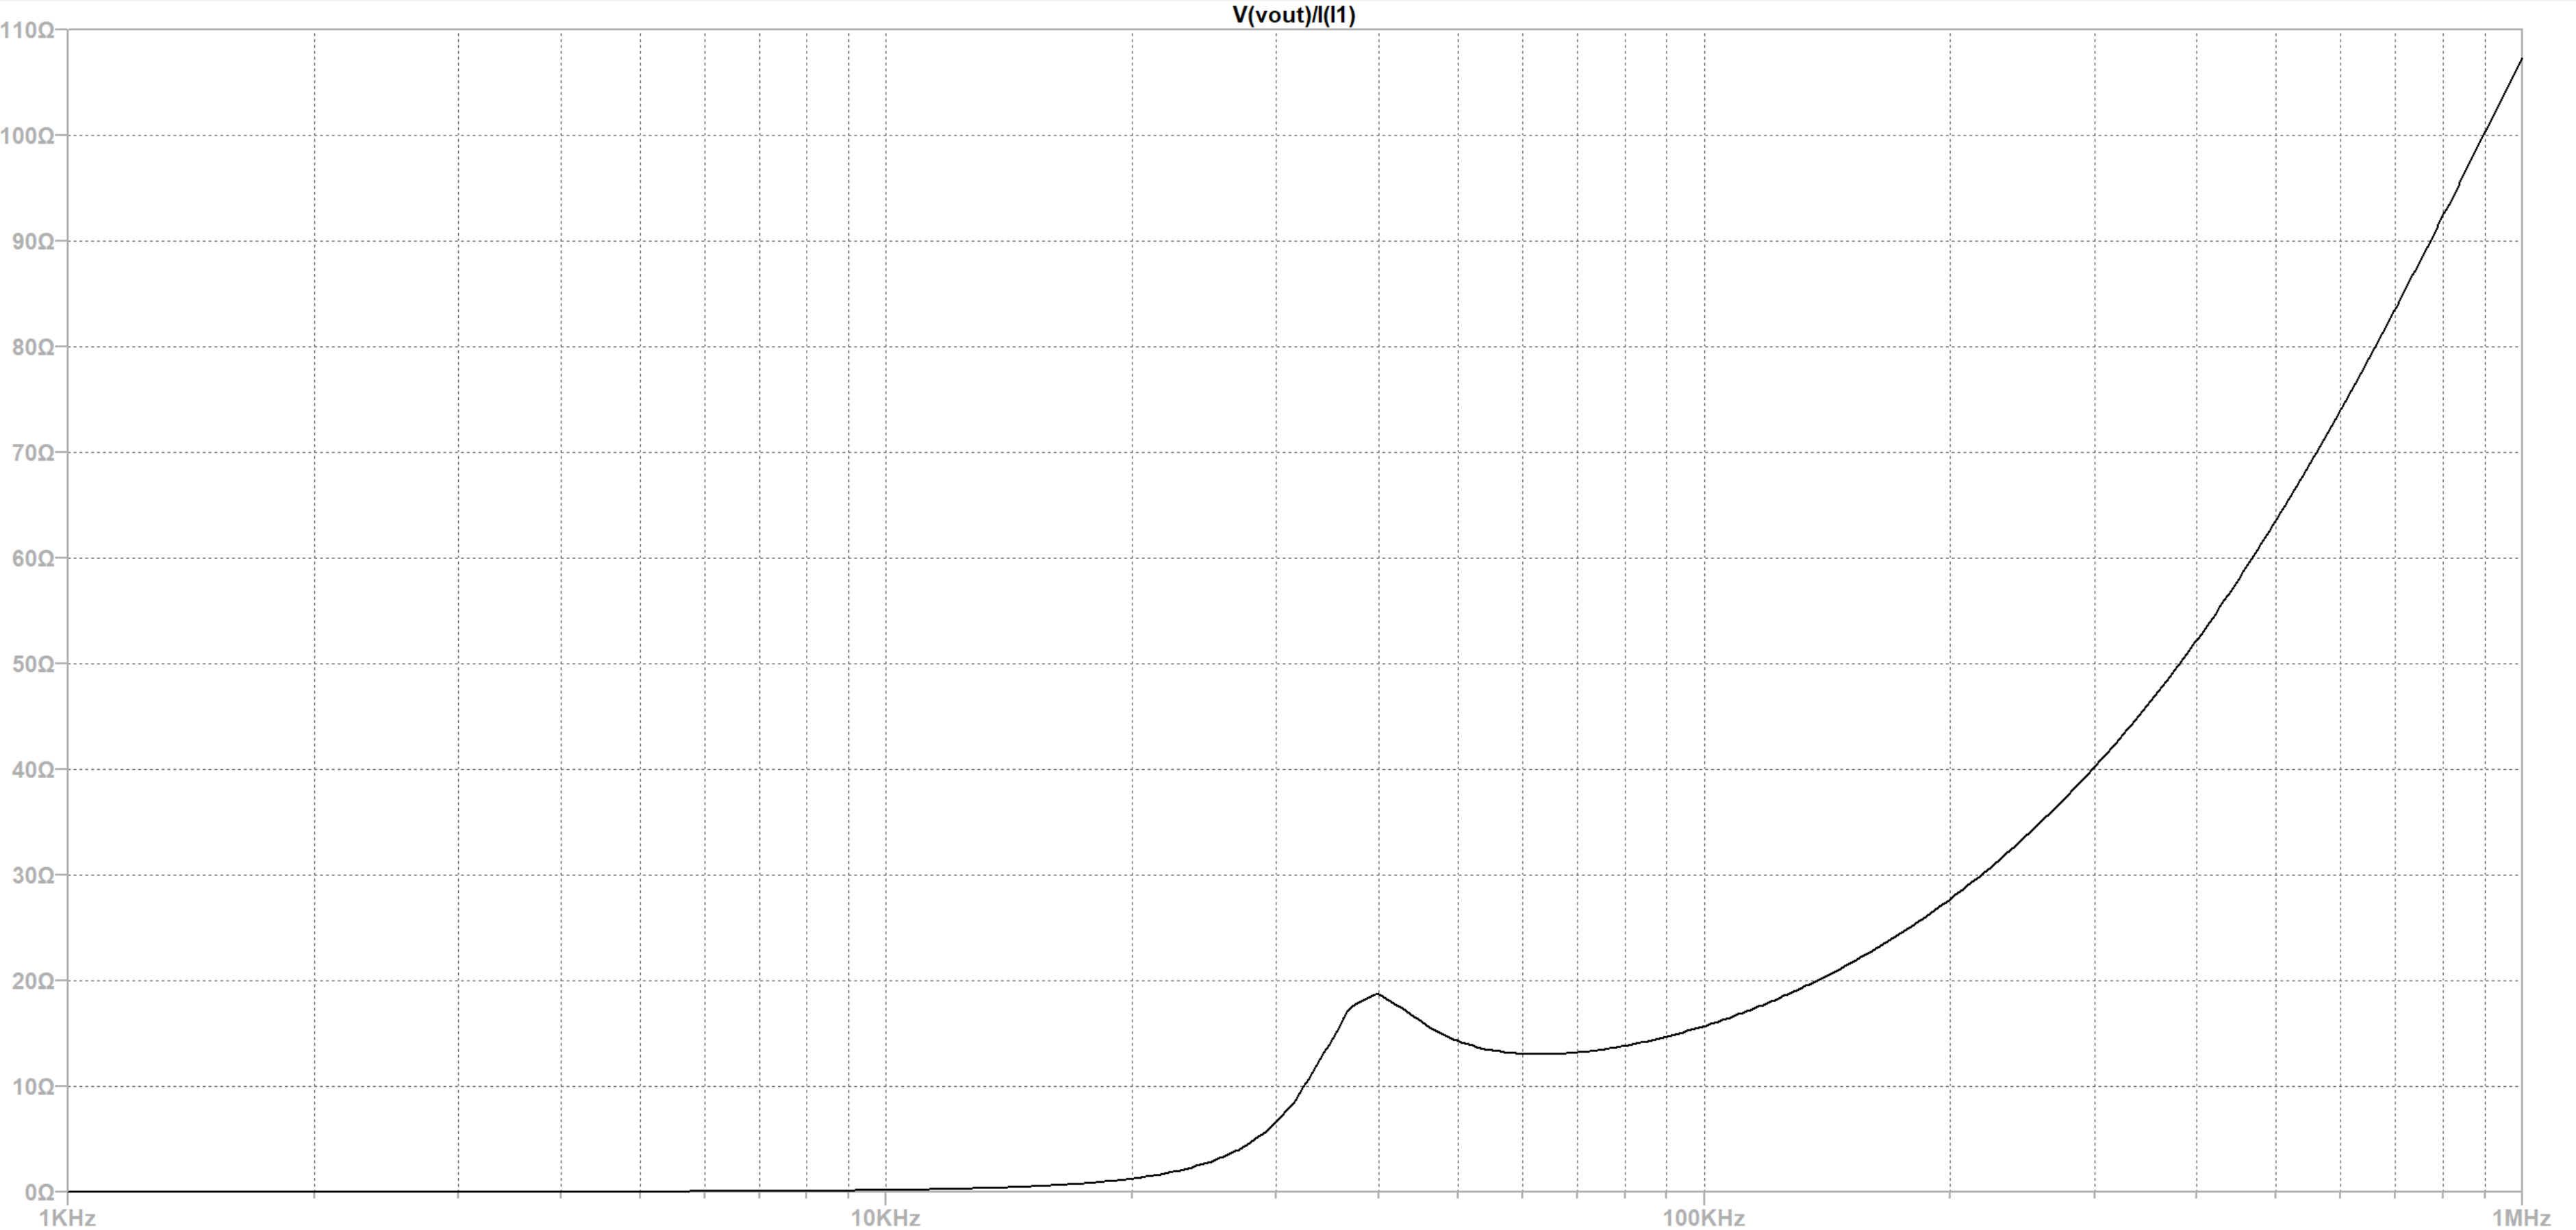
\includegraphics[width=0.9\textwidth]{../Ex4/Resources/ej4_impedancia_salida.png}
    \caption{Simulación de impedancia de salida}
    \label{fig:ej4_impedancia_salida}
    \end{figure}
    


\section{Medición}
En esta sección se muestran los resultados de las mediciones. Primero se exponen los bodes de las etapas por separado para poder determinar si cada etapa funciona de la manera esperada. En los bodes de las etapas se muestran tres curvas. La primera es la simulación con los componentes calculados (los de las tablas \ref{tab:ej4_e1_componentes_calculados} y \ref{tab:ej4_e1_componentes_calculados}), la segunda es con los componentes con los valores comerciales (los de las tablas \ref{tab:ej4_e1_componentes} y \ref{tab:ej4_e2_componentes}) y la tercera curva es la medición. Como ultimo se muestra el bode del filtro completo. En este se muestra la simulación de todo el filtro completo con los buffers a la entrada de cada etapa y su respectiva medición.  

El bode de la primera etapa se ve en la Figura \ref{fig:ej4_bode_e1}. Se puede observar que los resultados son sumamente satisfactorios ya que la simulación con los valores de los componentes calculados, la simulación con los valores de los componentes utilizados y la medición eso prácticamente idénticos. Esto sucede en la magnitud que es el parámetro de interés. También, nótese que en la medición y en la simulación la atenuación aumenta en frecuencias altas. Esto es de esperarse ya que a estas frecuencias comienza a actuar el polo dominante del amplificador operacional. En cuanto a la fase, se puede apreciar una cierta dispersión pero a partir de $100kHz$. La frecuencia donde se ubica el \textit{notch} es aproximadamente $29800 Hz$ lo que es excelente ya que es prácticamente igual a $f_{z1}$. Ademas, cabe aclarar que el preset en $R_7$ resulta de enorme ayuda ya que permitió ubicar el polo de la etapa en la frecuencia deseada dando muy buenos resultados. 

\begin{figure}[h!]                                                
    \centering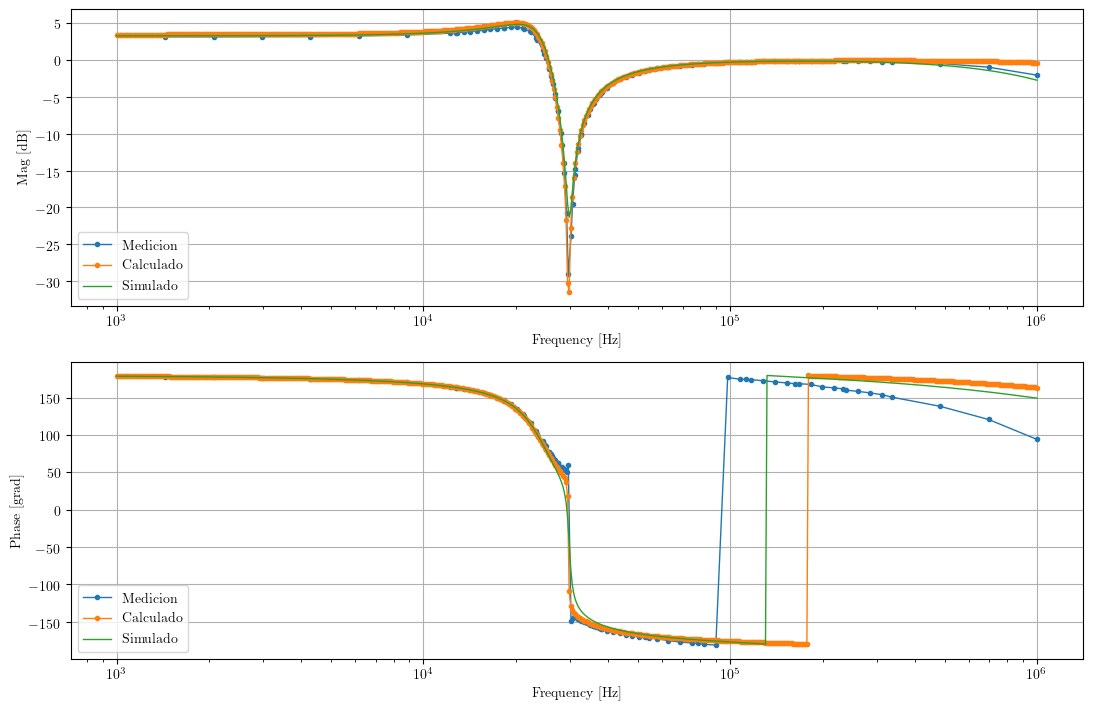
\includegraphics[width=0.9\textwidth]{../Ex4/Resources/ej4_bode_e1.png}
    \caption{Bode primera etapa}
    \label{fig:ej4_bode_e1}
    \end{figure}

Algo muy similar se dio en la segunda etapa. El bode de la misma se puede ver en la Figura \ref{fig:ej4_bode_e2}. Al igual que la primera etapa, los resultados son muy buenos. El \textit{notch} se ubica prácticamente en $f_{z2}$ y las tres curvas están prácticamente superpuestas.  

\begin{figure}[h!]                                                
    \centering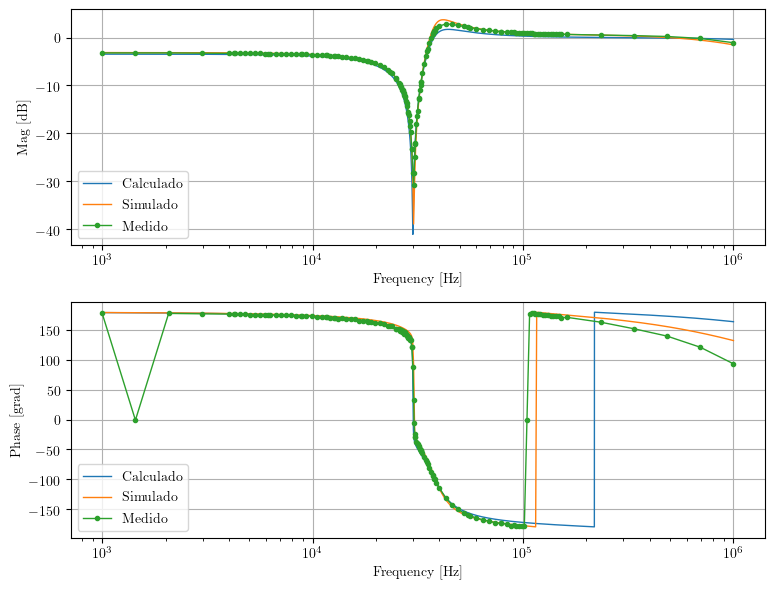
\includegraphics[width=0.9\textwidth]{../Ex4/Resources/ej4_bode_e2.png}
    \caption{Bode segunda etapa}
    \label{fig:ej4_bode_e2}
    \end{figure}

Finalmente, en la Figura \ref{fig:ej4_bode_completo} se muestra el bode del filtro con ambas etapas y sus respectivos buffers. Como era de esperarse la simulación y la medición son prácticamente iguales ya que las etapas por separado dieron muy buenos resultados. En primer lugar, se contempla que la frecuencia donde se ubica el \textit{notch} es muy aproximado a $30 kHz$ por lo que el filtro cumple dicho condición de la plantilla. Ademas, se logra una profundidad de \textit{notch} mayor a $50 dB$ cumpliendo la condición de la plantilla. También, se puede ver que se logra cumplir con el resto de las condiciones de la plantilla.   

\begin{figure}[h!]                                                
    \centering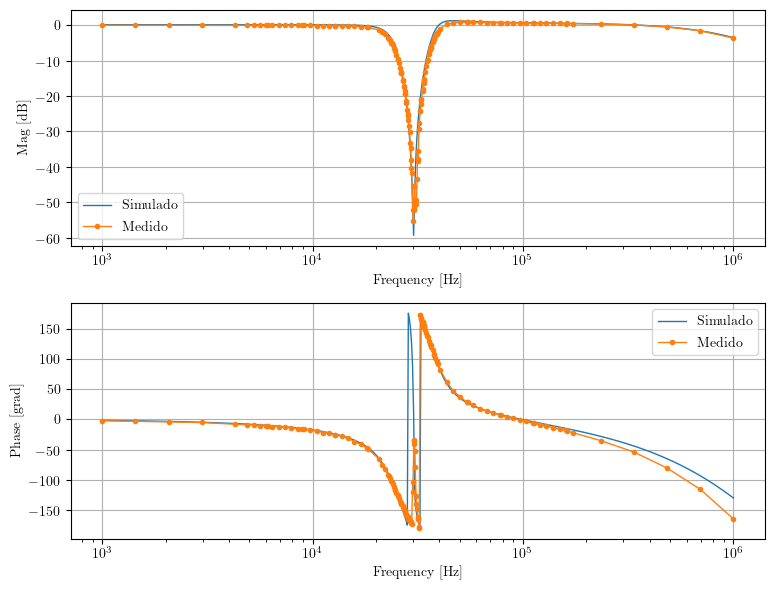
\includegraphics[width=0.9\textwidth]{../Ex4/Resources/ej4_bode.png}
    \caption{Bode del filtro}
    \label{fig:ej4_bode_completo}
    \end{figure}

\section{Conclusión}
Se logro implementar el filtro deseado con dos etapas con la configuración \textit{Fleischer-Tow}. La plantilla del filtro se cumple en el filtro implementado. La decisión de utilizar un preset en $R_7$ fue de inmensa utilidad ya que permitió calibrar las etapas por separado y obtener los resultados deseados. 


